\section{Profil}
\subsection{SRA}
\begin{frame}
  \frametitle{Anforderungen}
 Implementierung des Profils, das \underline{eingeloggten} Profil-Besuchern erlaubt:
 \bigskip
 \begin{itemize}
  \item Persönliche Daten des Benutzers einzusehen
  \item Den Benutzer zu kontaktieren(via Email)
  \item Ist der Benutzer Tutor, wenn ja, was macht er?
 \end{itemize}
 
\end{frame}
\begin{frame}
\frametitle{Formulierung}
 Daraus entstand für das SRA:
 \bigskip
  \begin{block}{F3:Schüler}
  Jeder Nutzer hat die Möglichkeit [...] sich [...] einzuloggen.
  Dadurch erhält er Zugriff auf seinen Privaten Bereich, in dem er seine [...] persönlichen Daten ändern kann.
  Die persönlichen Daten setzen sich aus Vorname, Nachname, Alter, Anschrift, Passwort und Kontaktdaten zusammen.
  Nutzername, Name, Vorname und Geburtsdatum sind von einer Bearbeitung ausgeschlossen.
  Es besteht die Option seinen Account zu löschen.
 \end{block}
\end{frame}

\subsection{SAD}
\begin{frame}
\frametitle{Überblick}
 Für einen Überblick mussten folgende Fragen gestellt werden:
 \begin{itemize}
  \item Welche Grundanforderungen sind nötig?
  \item Welche Technologien/Sprachen werden benötigt?
 \end{itemize}
\end{frame}
\begin{frame}
 \frametitle{Analyse}
 Für das eigene \underline{und} andere Profil wurden folgende Umsetztung ausgearbeitet:
 \begin{itemize}
  \item Es soll \underline{eine}(*.php) Datei, für alles was mit dem Profil zu hat, geben. Dazu gehören folgende Unterscheidungen:
    \begin{itemize}
     \item In seinem Profil soll man Daten ändern können
     \item andere Profile soll man anschauen können
     \item Verweis zum Tutorprofil
    \end{itemize}
  \item Die eingegebenen Daten im eigenen Profil müssen validiert werden
  \item Es soll eine Rückmeldung geben
 \end{itemize}
\end{frame}
\begin{frame}
 \frametitle{Technologien/Sprachen}
 Formular:
 \begin{itemize}
  \item HTML5 zur Eingabevalidierung
 \end{itemize}
 Skript
 \begin{itemize}
  \item PHP5
  \item einige Daten über Webaddresse übergeben
  \item Formulardaten mit Hilfe der POST-Technologie
 \end{itemize}
\end{frame}
\begin{frame}
 \frametitle{Formulierung}
  \begin{block}{F31}
   Der Schüler kann durch ausfüllen von HTML5 Formularen seine Profildaten bearbeiten, diese werden durch HTML5 validiert. Die Daten werden in der Datenbank über ein PHP-Skript geändert.
  \end{block}
\end{frame}

\subsection{Beispiel}
\begin{frame}
 \frametitle{Blick aufs Profil}
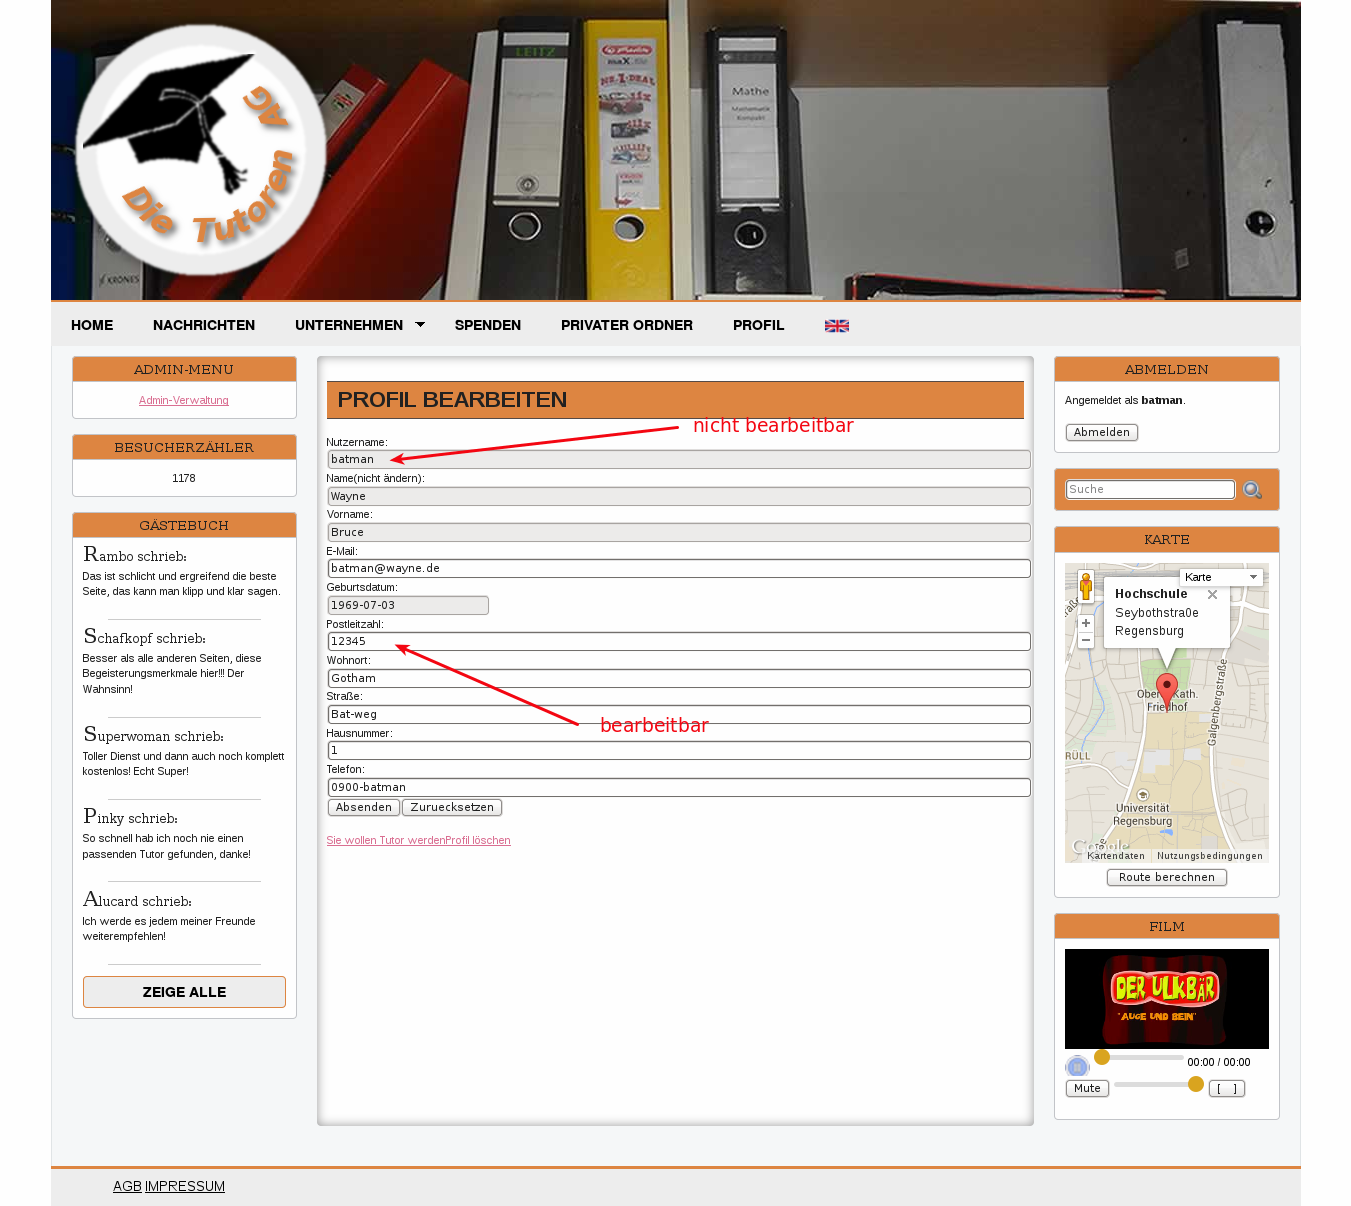
\includegraphics[width=1\textwidth]{./pictures/Profil-bearbeiten}
\end{frame}
\subsection{Implementierung}

\defverbatim[colored]
  \makeset{
    \phpcode

  \begin{lstlisting}[name=profile.php]
<?php
  if(isset($_SESSION['user']))
  {
    if(isset($_GET['DeleteProfile'])){...;}
    if(isset($_GET['value'])){...;}
    if(isset($_GET['password'])){...;}
    else
    {
       	include_once($_SERVER["DOCUMENT_ROOT"] . "/test_02/scripts/beeingTutor.php");
       	include_once($_SERVER["DOCUMENT_ROOT"] . "/test_02/scripts/GetProfile.php");
       	if(isset($result[0]))
       	{
       		$result = $result[0];
       		include_once($_SERVER["DOCUMENT_ROOT"] . "/test_02/scripts/getAllTutorData.php");
       		$umkreis = $AllTutorData[0]['umkreis'];
       		foreach($AllFachfromTutor as $fach)
       		{
       		    [Tabelleinhalt erstellen]
       		}
  \end{lstlisting}
}
  \begin{frame}
 \frametitle{Code}
 \begin{example}{profile.php}
  \makeset
 \end{example}
\end{frame}

\defverbatim[colored]
  \makeset{
    \phpcode
    
  \begin{lstlisting}[name=profile2.php]
          		include_once($_SERVER["DOCUMENT_ROOT"] . "/test_02/de/content/profile.html");   // Inkludiert static things
       	}
       	else  // this user doesn't exist
       		include_once($_SERVER["DOCUMENT_ROOT"] . "/test_02/de/content/noProfile.html");
      }
  }
  else
    [Fehlermeldung -> man ist nicht eingeloggt]
?>
  \end{lstlisting}
}
  \begin{frame}
 \frametitle{Code}
 \begin{example}{profile.php}
  \makeset
 \end{example}
\end{frame}
\defverbatim[colored]
  \makeset{
    \phpcode
      \begin{lstlisting}[GetProfile.php]
<?php
    include_once($_SERVER["DOCUMENT_ROOT"] . "/test_02/scripts/ConToDB.php"); // connection to DB
    $dbConnection = ConnectToDB();
    $dbConnection->setAttribute(PDO::ATTR_CASE, PDO::CASE_NATURAL);
    $query = $dbConnection->prepare("select * from mitglieder where benutzername = '" . $fl_username . "'");
    if($query->execute())
    {	
       $result = $query->fetchAll(PDO::FETCH_ASSOC);
       return $result;
    }
    else
       return null;
   $dbConnection = null;	// delete DB-Connection
?>
      \end{lstlisting}
}
\begin{frame}
 \frametitle{Code}
 \begin{example}{GetProfile.php}
  \makeset
 \end{example}

\end{frame}
\defverbatim[colored]
  \makeset{
    \phpcode
	\lstset{language=html}
      \begin{lstlisting}
<div class="scrollablecontentbox">
<h1>Profil <?php if($fl_username == $_SESSION['user']) echo "bearbeiten";?> </h1>

<form name="Formular" method="post" action="/de/profile.php?value=edit&username=<?php echo $_SESSION['user'];?>">
	<div><label for ="benutzername">Nutzername:</label><input type="text" size="45" maxlength = "45" value="<?php echo $result["benutzername"];?>" id="benutzername" name="benutzername" required readonly></div>
	[andere Formulardaten]
</form> 

<?php if($result["benutzername"] != $_SESSION['user']) echo '<a href="mailto:' . $result["email"] . '"><img src="/images/mail.png" alt="mail"> </a>'; ?>
[weitere Abfragen zur Tutorinformation]
<?php if($fl_username == $_SESSION['user']) echo '<a class="btn" href="/de/profile.php?DeleteProfile=true">Profil loeschen</a>'; ?>
<?php if(($tutor_result) and ($fl_username != $_SESSION['user']))
  [Tutorinformationen]
?>
</div>
      \end{lstlisting}
}
\begin{frame}
 \frametitle{Code}
 \begin{example}{Profil-Formular}
  \makeset
 \end{example}

\end{frame}
